\documentclass{article}
\usepackage[utf8]{inputenc}

\title{Smart Auctions}
\author{Andrea Bongiorno}
\date{June 2019}

\usepackage{natbib}
\usepackage{caption}
\usepackage{graphicx}
\usepackage{pgf}
\usepackage{tikz}
\usetikzlibrary{arrows,automata}
% Copyright 2017 Sergei Tikhomirov, MIT License
% https://github.com/s-tikhomirov/solidity-latex-highlighting/

\usepackage{listings, xcolor}

\definecolor{verylightgray}{rgb}{.97,.97,.97}

\lstdefinelanguage{Solidity}{
	keywords=[1]{anonymous, assembly, assert, balance, break, call, callcode, case, catch, class, constant, continue, constructor, contract, debugger, default, delegatecall, delete, do, else, emit, event, experimental, export, external, false, finally, for, function, gas, if, implements, import, in, indexed, instanceof, interface, internal, is, length, library, log0, log1, log2, log3, log4, memory, modifier, new, payable, pragma, private, protected, public, pure, push, require, return, returns, revert, selfdestruct, send, solidity, storage, struct, suicide, super, switch, then, this, throw, transfer, true, try, typeof, using, value, view, while, with, addmod, ecrecover, keccak256, mulmod, ripemd160, sha256, sha3}, % generic keywords including crypto operations
	keywordstyle=[1]\color{blue}\bfseries,
	keywords=[2]{address, bool, byte, bytes, bytes1, bytes2, bytes3, bytes4, bytes5, bytes6, bytes7, bytes8, bytes9, bytes10, bytes11, bytes12, bytes13, bytes14, bytes15, bytes16, bytes17, bytes18, bytes19, bytes20, bytes21, bytes22, bytes23, bytes24, bytes25, bytes26, bytes27, bytes28, bytes29, bytes30, bytes31, bytes32, enum, int, int8, int16, int24, int32, int40, int48, int56, int64, int72, int80, int88, int96, int104, int112, int120, int128, int136, int144, int152, int160, int168, int176, int184, int192, int200, int208, int216, int224, int232, int240, int248, int256, mapping, string, uint, uint8, uint16, uint24, uint32, uint40, uint48, uint56, uint64, uint72, uint80, uint88, uint96, uint104, uint112, uint120, uint128, uint136, uint144, uint152, uint160, uint168, uint176, uint184, uint192, uint200, uint208, uint216, uint224, uint232, uint240, uint248, uint256, var, void, ether, finney, szabo, wei, days, hours, minutes, seconds, weeks, years},	% types; money and time units
	keywordstyle=[2]\color{teal}\bfseries,
	keywords=[3]{block, blockhash, coinbase, difficulty, gaslimit, number, timestamp, msg, data, gas, sender, sig, value, now, tx, gasprice, origin},	% environment variables
	keywordstyle=[3]\color{violet}\bfseries,
	identifierstyle=\color{black},
	sensitive=false,
	comment=[l]{//},
	morecomment=[s]{/*}{*/},
	commentstyle=\color{gray}\ttfamily,
	stringstyle=\color{red}\ttfamily,
	morestring=[b]',
	morestring=[b]"
}

\lstset{
	language=Solidity,
	backgroundcolor=\color{verylightgray},
	extendedchars=true,
	basicstyle=\footnotesize\ttfamily,
	showstringspaces=false,
	showspaces=false,
	numbers=left,
	numberstyle=\footnotesize,
	numbersep=9pt,
	tabsize=2,
	breaklines=true,
	showtabs=false,
	captionpos=b
}	

\begin{document}

\maketitle
\newpage
\tableofcontents
\newpage
\section{Introduction}
The final term of the \textit{Peer to Peer and Blockchain} course requires to develop two different Solidity's smart contracts implementing different kind of auctions. For this project I have implemented the \textit{English Auction} and the \textit{Vickrey Auction}.

I decided also to implement a little escrow mechanism with the aim to highlight the problem of trust in the e-commerce world, it is described in Section \ref{escrow}. In Section \ref{vickrey}, \ref{english} respectively are described the two auction's implementations.

Since an e-commerce system is quite a critical one, I used some well defined programming pattern to achieve an high degree of security, they are illustrated in Section \ref{security}.

In the end, the Section \ref{gas} estimates the gas consumption of typical interactions between users and contracts developed.  
\section{Contracts}
\subsection{Escrow}\label{escrow}
Since this project aims to model online auctions and given the technology used, there is no trust between the main actors involved: seller and buyers.
In order to fill this trust gap has been implemented a little escrow contract, contained into the file Escrow.sol, with the purpose of protecting both seller and buyer but keeping in mind that when a bid is made, the buyer immediately sends its money.

Using the following real world analogy, here is the rationale behind this escrow contract. The actors involved are: the seller who has the responsibility to send the good, the buyer, the auctioneer who act as a referee, and a courier chosen by the seller. Here is a step-by-step scenario:
\begin{itemize}
    \item The winning buyer, after the conclusion of the auction, sends to the auctioneer, the SHA3 of a chosen nonce.
    \item The seller cannot deliver the good directly to the buyer, so he will use a third party courier.
    \item When the courier arrives at buyer's place, he will deliver the good only if the buyer reveals the correct nonce. 
    \item The seller receives the nonce from the courier so he can prove to the auctioneer the correct deliver of the good and then get paid.
    \item Now, two scenarios are open:
    \begin{enumerate}
        \item The buyer refuse to reveal the nonce or collude with the courier: in this case if the seller can prove to the auctioneer that he has sent the good (e.g. with an expedition number) then he get paid. Note that this scenario is unlikely because the buyer has already paid when making the winning bid.
        \item The seller doesn't send the good: in this case he won't be able to prove the expedition and the buyer will be refunded.
    \end{enumerate}
\end{itemize}

Obviously the escrow mechanism illustrated above is more a proof of concept than a practical solution, but I decided to implement it anyway in order to highlight the problem of trust with e-commerce.
\subsection{Auction}
Into the file Auction.sol is defined a \textit{super-contract} that encapsulates some common features between the Vickrey auction and the English Auction.
This contract contains:
\begin{itemize}
    \item Events, used by the sub-contracts to notify the occurrence of some facts such new offers, auctions' state, withdrawals and refunds.
    \item Common state variable, such as seller and buyer addresses, reserve price of the good, initial and final block of the auction.
    \item Debug variables, used to bypass modifier when debugging.
\end{itemize}

Both the auctions implemented are modelled as a state machine, following the corresponding behavioural pattern described in Section \ref{statemachine}.
\subsubsection{Vickrey Auction}\label{vickrey}
For this auction, in the real-world, bidders commit their offers in a sealed envelope, they have the possibility to withdraw their offer before the opening phase.
In the proposed implementation, has been chosen to model the bids from the bidders using a struct composed by the following field:
\begin{itemize}
    \item \textit{bidHash}: a bytes32 that represents the sealed envelope.
    \item \textit{value}: the actual value of the bid, this field will be filled once the envelope is opened.
    \item \textit{opened, withdrawn, refunded}: three booleans that describe the state of the bid.
\end{itemize}
The bids are collected into a mapping using as key the address of the corresponding bidder.

This implementation propose a state machine view of the Vickrey auction. The several states are described by the enum \textit{Phases} and they are the following:
\begin{enumerate}
    \item Commitment
    \item Withdrawal
    \item Opening
    \item Finished
\end{enumerate}
with the obvious semantics. 

The phases listed above follow each other temporally (without overlapping) and the flow of time has been implemented using the modifier \textit{blockTimedTransition}: it checks if the actual block number allows a state transition, according to the parameter provided at deploy time. For sake of completeness, the function is reported in Listing \ref{timevickrey}. The modifier \textit{duringPhase} checks if a certain function it's called in the correct phase. These modifiers are part of the \textit{State Machine pattern}.

\begin{lstlisting}[language=Solidity, caption={Modifier used for modelling the time flow during a Vickrey auction. The function \textit{nextPhase()} realise the transition from the actual phase to the next one, following the order described above and emitting an event.},captionpos=b, label=timevickrey]
modifier blockTimedTransition() {
    if(phase == Phases.Commitment && block.number > end_commitment)
        nextPhase();
    if(phase == Phases.Withdrawal && block.number > end_withdrawal)
        nextPhase();
    if(phase == Phases.Opening && block.number > end)
        nextPhase();
    _;
}
\end{lstlisting}

The three main phases of the Vickrey auction are controlled mainly by three functions:
\begin{enumerate}
    \item \textit{commit}: this function takes a bytes32 as parameter, it is the \textit{keccak-256} of a nonce concatenated to the value of the bid. Everyone can commit a bid, but it is allowed only one bid for bidder. When invoking this function, the bidder must send a deposit. The deposit requirement is set at contract construction by the auctioneer and it must be between a half and a quarter of the reserve price. On success this function emit a \textit{LogEnvelopeCommitted} event, with the address of the bidder as parameter.
    \item \textit{withdrawEnvelope}: using this function a bidder that has previously committed a bid and has not withdrawn it yet, can withdraw it. In this case the bidder will immediately receive a refund equal to half of the deposit requirement. Since the bidder receiving the refund is the one who call the function, an immediate refund does not violate the \textit{Withdrawal pattern} described in \ref{withdrawal}. The state of the bid is updated, setting to \textit{true} the corresponding field.
    \item \textit{open}: this function can be invoked only once from a bidder that has not withdrawn his envelope. The bidder sends as parameter the nonce used to calculate the \textit{bidHash} along with its actual bid. These values are used to calculate a \textit{keccak-256} to be compared with the one previously sent. On failure the transaction is reverted, on success there are the following possibilities:
    \begin{enumerate}
        \item The bid is less than the reserve price: this case is treated as cheating because the bidder made an offer knowing that it cannot be the winning one. In this case the bidder will receive a refund of his bid and a half of the deposit requirement. A \textit{LogVoidBid} with information about the bidder and the bid is emitted.
        \item The bid is the first one: in this case the price to pay (second highest bid) is set to reserve price and information about the bidder and the bid are recorded into the variables \textit{highestBid} and \textit{highestBidder}. A \textit{LogHighestBid} event is emitted.
        \item The bid is lower than the highest bid: the value of the bid is checked against the second highest bid and if it is greater then the price to pay is updated and also a \textit{LogUpdateSecondPrice} is emitted. Anyway, the bidder will receive a full refund (deposit + bid value) and a \textit{LogLosingBid} is emitted. Again, the \textit{Withdrawal pattern} is not violated and the status of the bid is updated to \textit{refunded}.
        \item The bid is the new highest one: when this situation occurs the price to pay is updated to the old highest bid and the new information about the actual highest bid and highest bidder are also updated. Is not possible to refund immediately the previous highest bidder because in this case the \textit{Withdrawal pattern} will be violated, as explained deeply in \ref{withdrawal}.
    \end{enumerate}
\end{enumerate}

When the opening phase is ended, and the contract is in the \textit{Finished} state, there are two things left: finalize the auction and refund bidders that weren't refunded during the opening phase.
The refund is performed using the function \textit{getRefund} that can be called only once by those bidders that opened their envelope and has not received a refund yet (check point d of the list above). This function was written just to implement the \textit{Withdrawal pattern} described in \ref{withdrawal}, if it is called by the highest bidder than he will receive as refund the entire deposit plus the difference between his bid and the second highest bid, otherwise the bidder who call this function will receive as refund the deposit plus his bid.

For what concern the finalization of the auction there is a function \textit{finalize} that can be called only once by the auctioneer. This function does two things: first it deploy an escrow contract and second transfer the funds of bad bidders to a charity address specified at the construction of the auction's contract. If this method is called passing \textit{true} as parameter, a \textit{LogEscrow} event is emitted, which contains the address of the escrow contract. If there aren't valid bid, the good remains unsold and a \textit{LogUnsold} event is emitted.

\subsubsection{English Auction}\label{english}
Also this auction has been modelled as a state machine but in a slightly different way with respect to the previous one. The possibile states are described by the struct \textit{Phases} and they are the following:
\begin{enumerate}
    \item Started,
    \item BidReceived,
    \item Sold,
    \item Finished
\end{enumerate}

For this auction the states does not follow each other temporally and the state transitions are described by the automaton below.
\begin{center}
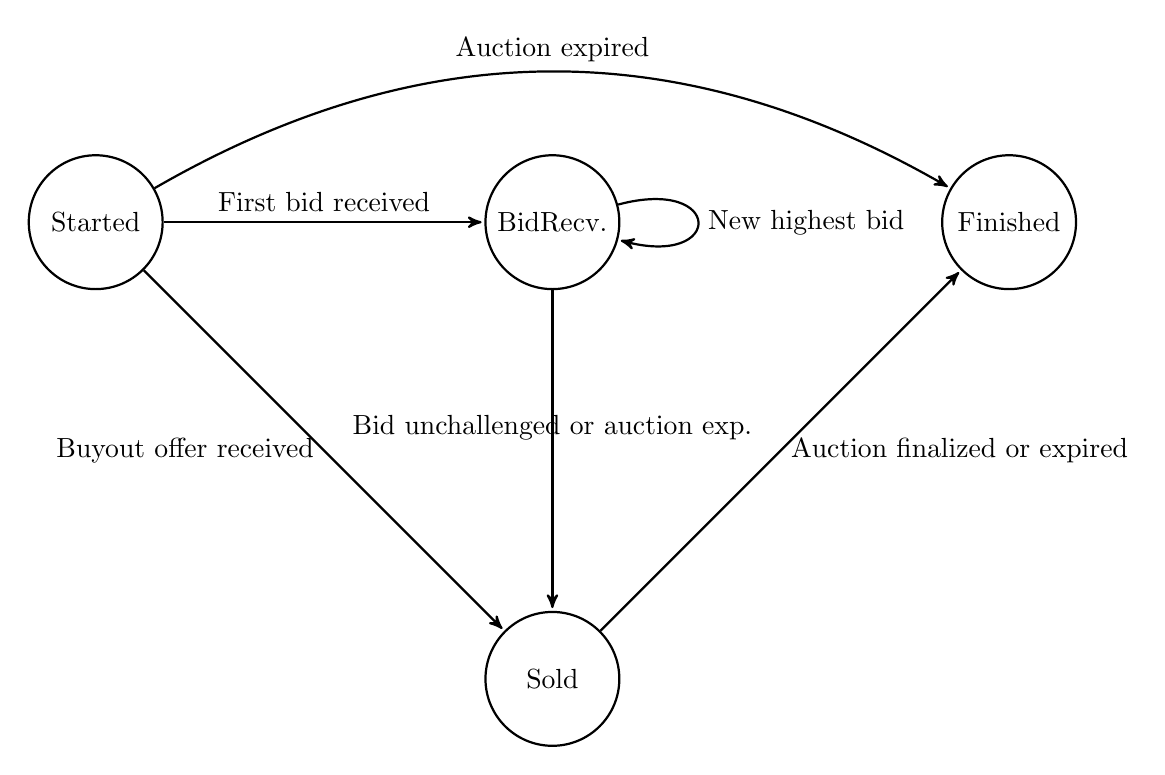
\begin{tikzpicture}[->,>=stealth',shorten >=1pt,auto,node distance=5.8cm,thick]\label{englishstates}
  \tikzstyle{every state}=[fill=white,text=black]

  \node[state, minimum size=1.7cm]         (A)                    {Started};
  \node[state, minimum size=1.7cm]         (B) [right of=A]       {BidRecv.};
  \node[state, minimum size=1.7cm]         (C) [below of=B]       {Sold};
  \node[state, minimum size=1.7cm]         (D) [right of=B]       {Finished};

  \path (A) edge [above]      node {First bid received} (B)
            edge [left]       node {Buyout offer received} (C)
            edge [bend left]  node {Auction expired} (D)
        (B) edge [loop right] node {New highest bid} (B)
        (B) edge [above]      node {Bid unchallenged or auction exp.} (C)
        (C) edge [right]      node {Auction finalized or expired} (D);
\end{tikzpicture}
\end{center}

Once again the flow of time has been implemented using the modifier \textit{blockTimedTransaction}, that is slightly different from the previous one, as shown by Listing \ref{englishtime}.

\begin{lstlisting}[language=Solidity, caption={Modifier used for modelling the time flow during an English auction, according to the automaton.},captionpos=b, label=englishtime]
 modifier blockTimedTransition {
    if(phase == Phases.BidReceived && (block.number > end || block.number > bidBlock+unchallengedInterval)) {
        phase = Phases.Sold; 
        emit LogSold(highestBidder, highestBid);
    }
    else if(phase == Phases.Started && block.number > end) {
        phase = Phases.Finished;
        emit LogPhaseTransition("Finished");
    }
    _;
}
\end{lstlisting}

The main operations available for this kind of auction are the following:
\begin{itemize}
    \item \textit{buyNow}: it can be invoked only in the \textit{Started} phase and its successful execution triggers a transition to the \textit{Sold} state. When invoking this function, the buyer has to provide the exact amount for the buyout, established at contract deploy. This function cannot be invoked if a bid has been already received i.e. if the contract is in the \textit{BidReceived} state, as required by the text of the assignment.
    \item \textit{bid}: this is the function for bidding. A bid is valid if it is made in the \textit{Started} phase or in \textit{BidReceived} phase (when the \textit{unchallenge period} is not expired yet). The bid must be greater than the previous one plus a minimum increment specified, in percentage, at contract deploy time and stored in the variable \textit{minIncrement}. Obviously, in the case of the first bid of the auction, this function triggers a phase transition form \textit{Started} to \textit{BidReceived}.
    \end{itemize}

When a bid is outbid, there is one bidder that has to be refunded: this cannot be done inside the \textit{bid} function because this would violate the \textit{Withdrawal pattern}. If a bidder wants to be refunded, he can call the \textit{withdrawal} function and get a refund.

\section{Security consideration}\label{security}

Since for this project there are theoretically some money involved, guarantee the security of the systems developed is not trivial. The main risk when programming in \textit{Solidity}, excluding trivial bugs, is the re-entrancy attack: when a contract interacts with another one (e.g. when transferring funds) it has to consider the possibility that the called contract can re-call it and this can result in bad behaviour such double-spending of some kind of token or funds, or denial of service.
In this section are described three widely used design patterns that if well implemented they guarantee an high level of protection from attacks and misbehaviour. 
\subsection{State Machine pattern}\label{statemachine}
The State Machine pattern is a behavioural pattern, useful to model systems that can be in several state with well defined rules for the transitions between states.
Contracts that fit in this scheme are often characterised by the fact that they expose certain functionality only when they are in a precise state.

This pattern when well implemented ensure that the contract exposes only the correct functionality and guarantee consistency between the different states.

Auctions are a typical scenario where this pattern is used since they are often divided into stages and at each stage the bidders are allowed to execute only certain functions. Stages in auctions are controlled by time: in this case the State Machine pattern ensures soundness in the time flow: this is the rationale behind the modifiers \textit{blockTimedTransition} and \textit{duringPhase}, note that they must follow this order.

Implementation details for this pattern are not standard although it is very common the use of enum and struct for modelling the state and of modifiers in order to determine function exposure. The details for the code developed for this project have been described in Section \ref{english} and Section \ref{vickrey}.
\subsection{Withdrawal pattern}\label{withdrawal}
The Withdrawal pattern is a security pattern commonly used to send funds after an effect. Although it can be counterintuitive, this pattern is very powerful when the aim is to prevent a failure during a refund.

In order to understand its power let consider the following scenario. 
During an English auction, a dishonest bidder want to spend the least possible amount of ether to buy the selling good. To reach its goal the bidder make the first offer from an address associated with a contract. Next, another bidder makes his bid, higher than the one of the briber. Without using the withdrawal pattern the code executed will be something similar to Listing \ref{badeng}.

\begin{lstlisting}[language=Solidity, caption={Buggy code that do not use the withdrawal pattern},captionpos=b, label=badeng]
 function bid(...) ... {
    ...
    if(msg.value > highestBid) {
        /* refund the previous bidder*/
        highestBidder.transfer(highestBid);
        /*update info about winning bid*/
        highestBidder = msg.sender;
        highestBid = msg.value;
    }
    ...   
}
\end{lstlisting}

The problem is in line 5: \textit{highestBidder} contains the address of a contract owned by the briber and if this contract has a fallback function (called by \textit{transfer}) that always fails, it will be not possible to record an offer that outbid the one of the briber and the contract is trapped in its state. When the auction ends, the briber win the good spending the minimum amount of ether.

To implement the withdrawal pattern it is sufficient to remember who has to be refunded, for example using a mapping. When a bidder wants to withdraw his funds, he can call a specific function that make the transfer. Since the function is called by the owner of the funds, an eventual failure will only prevent the owner to recover its funds. A correct example is shown in Listing \ref{goodeng}, that differs from the previous only for line 5.

\begin{lstlisting}[language=Solidity, caption={Correct code that do use the withdrawal pattern},captionpos=b, label=goodeng]
 function bid(...) ... {
    ...
    if(msg.value > highestBid) {
        /* refund the previous bidder*/
        pendingRefunds[highestBidder] += highestBid;
        /*update info about winning bid*/
        highestBidder = msg.sender;
        highestBid = msg.value;
    }
    ...   
}
\end{lstlisting}

In the code developed, this pattern has been implemented for the English auction as shown by the above example and for the Vickrey auction because of the situation when the opening of an envelope outbid a previous winning bid.  

\subsection{Checks-Effects-Interactions pattern}\label{CEIpattern}
This security pattern has to be used when it cannot be avoided to hand over control flow to an external entity and it is desired protection against re-entrancy attacks. The C-E-I pattern is implemented in three steps:
\begin{enumerate}
    \item Check the eligibility of the function invocation.
    \item Adopt an \textit{optimistic accounting} policy by updating the state of the contract before a possible interaction with an external contract.
    \item Interact with the external contract.
\end{enumerate}
Is possible to find a perfect example of the C-E-I pattern considering the withdrawal pattern described in Section \ref{withdrawal}.

Once implemented the withdrawal pattern we have the be sure that a bidder can ask its refund exactly once. The intuitive solution is to implement a \textit{refund} function like the one in Listing \ref{badrefund}.

\begin{lstlisting}[language=Solidity, caption={Buggy refund function, vulnerable to re-entrancy attacks},captionpos=b, label=badrefund]
 function refund() public {
    require(pendingRefunds[msg.sender] > 0)
    
    msg.sender.transfer(pendingRefunds[msg.sender]);
    
    pendingRefunds[msg.sender] = 0;
}
\end{lstlisting}

Now, the function \textit{refund} respect the check-first property but the effects, i.e. zeroing the balance of \textit{msg.sender}, are performed after the interaction with an external contract. In such a situation if the \textit{transfer} in line 5 triggers a re-entrancy attack (through the fallback function) to the \textit{refund} function, \textit{msg.sender} will receive a double refund since its balance has not been updated yet.

The correct implementation is simple and requires just to swap line 4 with line 6. As a rule of thumb, when implementing this pattern, interactions (e.g. transfer, send, call etc.) should be the last commands of a function. Obviously in some cases a fail-safe policy should be implemented: if instead of \textit{transfer} I had used \textit{send}, on failure I had to update again the balance of \textit{msg.sender}.

For sake of completeness in Listing \ref{goodrefund} is shown the correct code.

\begin{lstlisting}[language=Solidity, caption={Correct refund function. Since on failure \textit{transfer} revert the transaction there is no need to check its returned value.},captionpos=b, label=goodrefund]
 function refund() public {
    require(pending_refunds[msg.sender] > 0)
    
    uint refund = pending_refunds[msg.sender];
    pending_refunds[msg.sender] = 0;
    
    msg.sender.transfer(refund);
}
\end{lstlisting}

\section{Gas consumption consideration}\label{gas}
In this section are provided some estimations of the gas needed for typical sequences of operations that a bidder does when interacting with the two contracts. In the considerations below will be used the following constants:
$$ B=21000, T=2300.$$
The constant above are respectively the base cost of a transaction and the cost of a \textit{transfer}.

Another useful constant for these estimations is $$L=1850$$ that is an estimation based on several execution of the cost of the primitive LOG1 with 3 arguments of 32 bytes each. A LOG1 is the main primitive used when emitting an event. The constant $L$ has been chosen in order to consider the worst case: not all the event emitted have 3 parameters.

The last two constants are the following: $$S=20000, S'=5000$$ they are respectively the cost of an SSTORE that update a value changing its \textit{zeroness} and the cost of an SSTORE that does not change the \textit{zeroness} of the value updated. 

For the following calculations are assumed successful invocations of the involved functions and a good behaviour of the bidders. Given the assumptions above, in many case will be possible to leave out the cost of modifiers since they perform comparisons (operations LT, GT, ISZERO etc) and conditional jumps (operations JUMP and JUMPI) that have a lower cost with respect to other operations performed by the functions.

Note: experiments shown that the effective gas consumption can be higher than the estimations in certain situations because of the timed nature of the code: one function call could trigger a state transition, this in turn triggers event and function calls. Is not so fair that this gas is paid by the bidder, one solution can be to enclose this code between \textit{msg.gas} calls and at the end calculate a refund for the caller.

\subsection{Vickrey auction scenario}
In the case of a Vickrey auction there are two main scenarios:
    \begin{itemize}
        \item \textit{Commit and Withdrawal}: \textit{commit} stores an hash into an entry of a mapping and emit an event. Storing the hash is a first-time write so its cost is $S$. In this scenario, when \textit{commit} terminates, \textit{withdrawEnvelope} is called by the bidder. This function does 3 operations: update the status of the caller's bid, refund the caller, emit an event. First main operation is again an SSTORE that costs $S$ gas units like above because we are setting to true (a non-zero value) the \textit{withdrawn} field of the bid that was false (a zero value). Second operation is the refund that costs $T$ and third operation is the event with cost $L$. Finally this sequence of operations will cost to a bidder $\approx 2\times (B + L + S) + T.$
        \item \textit{Commit and Open}: the commit cost is the same of the above scenario ($B+S+L$). The \textit{open} function has some fixed costs: some gas is consumed for computing a \textit{keccak} to check the validity of the bid (its cost is irrelevant and less than 50 gas, exactly 30 + 6 for each word, and we have 2 words so it's 42 gas) and $2\times S$ not negligible gas units for updating the bid status (two SSTORE that change the zeroness of the previous values of the fields \textit{opened} and \textit{value}). \textit{Open} can successfully terminate in three ways:
        \begin{enumerate}
            \item The opened bid is less than reserve price: this cost $S$ for updating the status of the bid into the mapping (the field \textit{refund} is set to true), $L$ for logging and $T$ for a partial refund.
            \item The opened bid is the first valid one: this cost $S \times 3$ for updating information about the price to pay, the highest bid and the highest bidder. In the end, an event is emitted paying $L$ gas units.
            \item The opened bid is a losing one: this may cost $S'$ gas unit plus $L$ if it is the new second highest (update \textit{priceToPay} and log) and also others $S$ for updating the bid status to refunded, $T$ for the actual refund and again $L$ for logging. In this case could be spent up to $S'+2\times L + T + S$ gas units.
            \item The opened bid is the new highest one: in this case the bidder pays $S' \times 3$ to update the variables that store information about the first and second highest bid (\textit{priceToPay, highestBid and highestBidder}), that cannot be zero, plus $L$ for logging.
        \end{enumerate}
        Summing up, the bidders pay a fixed amount of about $40000$ gas units that can go up to $140000$ (case 2), depending on the situation.
    \end{itemize}
    
According to \textit{ethgasstation.info}, at the time of writing
this report, commiting and opening a bid can cost up to 0.5 dollars, overestimating a gas consumption of 250000 gas units

\subsection{English auction scenario}
For the English auction the are two simple scenarios:
\begin{itemize}
    \item Buy now: in this case the bidder decide to buy the good by buyout. This case is simple and completely managed by the function \textit{buyNow} that costs $3\times S + L$: it updates the phase of the bid, the information about highest bid and highest bidder and emit an event for logging purpose. Note: the contract is passing from phase \textit{Started} to \textit{Sold}, since \textit{Started} is the first field of the enum \textit{Phases} its value is zero, instead the value of \textit{Sold} is two. 
    \item Bids: this scenario is divided in two cases: the bid received is the first one or it will be the new highest. 
    
    In the first case there is a first SSTORE on three zero variables: \textit{highestBid}, \textit{highestBbidder} and \textit{bidBlock}. Then is emitted an event and the contract goes to \textit{Sold} phase, for a total of $4 \times S + L$ gas units.
    
    In the second case the function is cheaper: non-zero information are updated for $3\times S'$, the refund for the previous highest bidder is saved, for $S$ gas units if is the first time his offer is outbid or for $S'$ otherwise.
\end{itemize}

\section{Testing guidelines}
In this section it is described how to test the two contracts implemented. For this purpose each contract has a variable, \textit{debug}, that if it's set to true at construction time it will disable the modifier \textit{blockTimedTransaction} and allow to manually switch between phases through the \textit{nextPhase} function. I assume that the contracts will be tested using Remix IDE.
\subsection{Testing Vickrey auction}
To test this contract follow the steps:
\begin{itemize}
    \item Deploy: the constructor has the following signature:
        \begin{lstlisting}[language=Solidity]
constructor (address payable _seller, address payable _charity, uint _reserve_price, uint _commitment_phase_length, uint _withdrawal_phase_length, uint _opening_phase_length, uint _deposit_requirement, uint _escrow_duration, bool _debug) public;
        \end{lstlisting}
        The parameters \textit{\_seller} and \textit{\_charity} can be freely chosen among the ones proposed by the IDE, keeping in mind that they are not allowed to commit a bid. The various \textit{*\_phase\_length} are intended to by number of blocks and they can be ignored when debugging or testing.
        \textit{\_deposit\_requirement} must be between one quarter and one half of \textit{\_reserve\_price}.
        
        An example call is the following:
        \begin{lstlisting}[language=Solidity]
constructor (..., ..., 1000 wei, 1, 1, 1, 500 wei, 50, true);
        \end{lstlisting}
    Note: this operation requires about 3,200,000 gas units.
    \item Execution: once the contract has been deployed it is in the \textit{CommitmentPhase}, follow the following steps to simulate the auction:
    \begin{enumerate}
        \item Choose one address, different from \textit{sender}, \textit{charity} and the one that deploied the contract (i.e. the auctioneer).
        \item Using the function \textit{debugKeccak} generate a hash, for example calling \textit{debugKeccak(0x01, 1000)} where the first value is a bytes32 nonce and the second is the bid promised.
        \item Using the hash of the previous step as paramter, call the function \textit{commit} and send also an amount equal to \textit{depositRequirement}, on success a \textit{LogCommitment} event is emitted.
        \item Go to step 1 and repeat as many time desired for send other commitment (up to one commitment per address).
        \item To switch to the withdrawal phase call the \textit{nextPhase} function with 1 as parameter, every time this function is called a \textit{LogTransition} is emitted.
        \item Call \textit{withdraw} function as many time as desired from the addresses used when committing. This function can be called only once for every address that committed. For every successful call an event is emitted.
        \item Once the withdrawals are finished, call \textit{nextPhase(2)} to switch to the \textit{OpeningPhase}.
        \item During the opening phase, who has not withdrawn at step 6 can open his envelope. In order to do this, choose a valid address and call the \textit{open} function providing as parameter the correct nonce used when the bid was committed. When calling this function send also the correct amount of ether for the bid. Depending on the order of opening different event could be emitted, they are described in Section \ref{vickrey}. Checking the value of the variables \textit{highestBidder}, \textit{highestBid} and \textit{priceToPay} is possibile to gain information about how the auction is going.
        \item Call \textit{nextPhase(3)} to switch to \textit{Finished} state. 
        \item Now, using the address of the auctioneer, the seller or the buyer is possible to call the function \textit{finalize} with a boolean as parameter. If the boolean is true than an escrow contract is deployed and its address is returned into a \textit{LogEscrow} event, otherwise an amout equal to \textit{priceToPay} is directely sent to the seller. In any case the funds left in the contract are sent to a charity address.
    \end{enumerate}
\end{itemize}
\subsection{Testing English auction}
To test this contract follow this steps:
\begin{itemize}
    \item Deploy: the constructor has the following signature:
        \begin{lstlisting}[language=Solidity]
constructor (address _seller, uint _duration, uint8 _min_increment, uint _buyout_price, uint _reserve_price, uint _unchallenged_interval, bool debug)
        \end{lstlisting}
        The parameter \textit{\_seller} can be freely chosen among the ones proposed by the IDE, keeping in mind that the seller is not allowed to commit bids. The parameter \textit{\_min\_increment} indicates the percentage of how greater a bid must be than the highest one in order to become the new highest whereas \textit{\_duration} and \textit{\_unchallenged\_interval} indicates respectively how many blocks lasts the auction and how many blocks are necessary before a bid is declared the winning one. The meaning of the others parameters is trivial, note that \textit{buyoutPrice} is required to be greater than \textit{reservePrice}.
        
        An example call is the following:
        \begin{lstlisting}[language=Solidity]
constructor (..., 50, 25, 1500 wei, 550 wei, 5, true);
        \end{lstlisting}
    \item Execution: once the contract has been deployed it is in the \textit{Started} phase, follow the following steps to simulate the auction:
    \begin{enumerate}
        \item Call the function \textit{buyNow} from an address different to the one of the seller or the one that deployed the contract (i.e. the auctioneer) if you want to terminate the auction by buyout. In this case if the correct amount is sent, the contract will switch to \textit{Sold} phase, as shown by the automata in Section \ref{english}. A \textit{LogSoldByBuyout} is emitted.
        \item If it has been chosen to not terminate the auction by buyout, select an address and call the function \textit{bid} with an amount at least equal to reserve price. Since this is the first bid, the contract will switch to \textit{BidReceived} phase.
        \item Do as many bid as desired, calling the \textit{bid} function with other addresses keeping in mind that the amount sent has to be greater than \textit{highestBid + (highestBid * minIncrement / 100)}.
        \item Since the flow of time has been locked using the \textit{debug} variable, when desired is possible to call \textit{nextPhase(2)} to switch to \textit{Sold} state, making the value stored in \textit{highestBid} the winning one.
        \item Now, whatever the auction is come to \textit{Sold} state, it his possible to call the method \textit{finalize} to end the auction. This method bring the auction to the \textit{Finished} state and if it is called with true as parameter it deploy an escrow contract just like the \textit{finalize} method of the Vickrey auction.
    \end{enumerate}
\end{itemize}

\appendix

\section{Auction.sol}

\section{Escrow.sol}

\section{VickreyAuction.sol}

\section{EnglishAuction.sol}

\end{document}